\pagestyle{fancy}

\chapter{Results and discussions}
\label{Chap4}

This part will present the results the measurements gave and the discussions we can have give according to these results.

\section{Room Temperature Results}
                \subsection{Reference Samples}
                
                Every experiment needs references to rely on. Before starting anything with the plasma, it is important to know the behaviour of the same structures (in terms of parameters) without plasma, to have access to a comparison. The three reference samples are a clean contact (Al/Cu), a strong oxidation reference (as a native oxidation imitation) (Al/Al Oxide/Cu) and a tunnel junction (Al/Al Oxide/Cu).
                
                The first junction is a clean contact with only Al and Cu as a reference. Since the contact is clean, the resistance of the interface between the two metals should be negligible, then the resistance we measure is :
                
                \begin{equation}
                  R=\sum_{Al,Cu}\dfrac{\rho L}{S}  
                  \label{loidohm}
                \end{equation}
                
                The resistance does not depends on the surface area of the junction, as you can see in Fig. \ref{cleancontact} the results of four probes measurements. As expected the resistance does not depend on the resistance of the surface of the junction.
                The theoretical calculus from this law with the parameters used gives $78\Omega$, which is close to the value we find. There are some uncertainties : the thickness of the metal is not very precise, the dimensions of the device can differ a bit from the pattern dimension. However, the order of magnitude is correct, so our reference for the leads resistance is around $70\Omega$.

                
                \begin{figure}
                    \centering
                    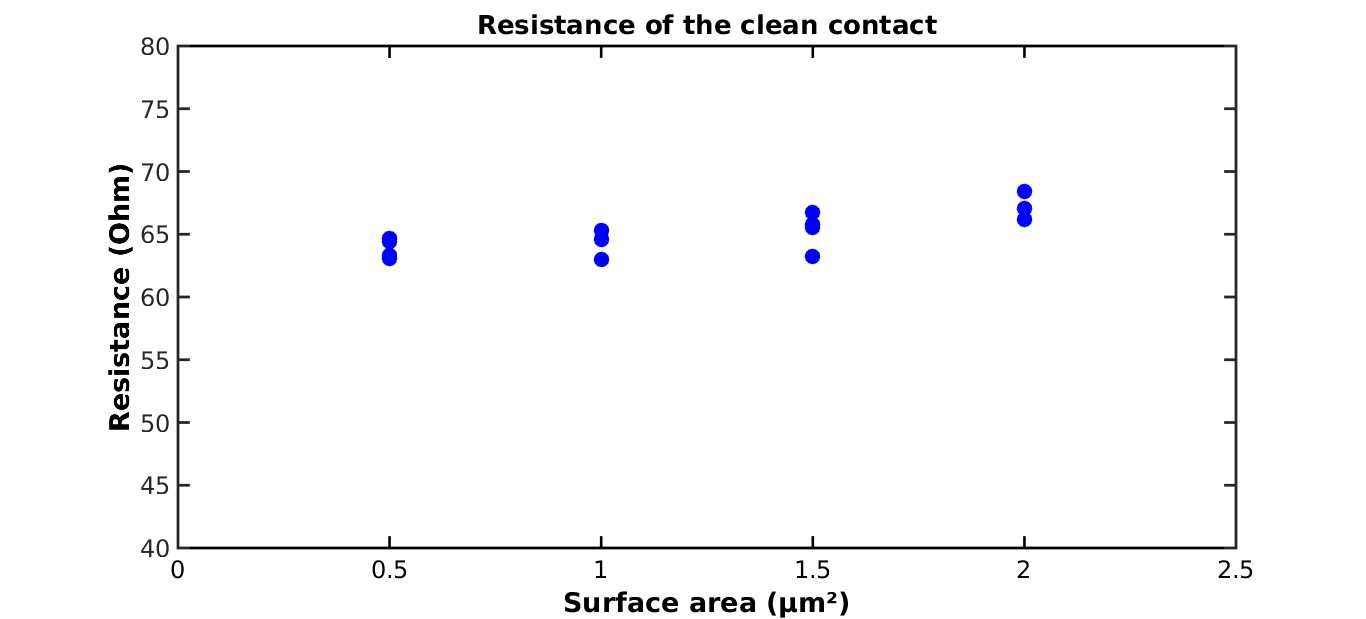
\includegraphics[width=15cm]{Rclean.png}
                    \caption{Resistance of clean contact in function of the surface area}
                    \label{cleancontact}
                \end{figure}
                
           
                After the clean contact, the second reference sample is with a strong oxidation (10 min at an oxygen atmosphere of 200mbar).

                For the NIS junctions, it is more relevant to draw conductance in function of the surface area of the junction. Indeed, the previous law (Eq. \ref{loidohm}) is correct for an insulator, except that $\rho_{AlOx}$ is order of magnitudes higher than $\rho_{Al}$ or $\rho_{Cu}$ and the surface of the junction is the surface of the insulator considered. The resistance of the device is mostly the resistance of the junction, and the conductance of the junction is linear with the surface. The measurements on these samples gave the conductance curve represented in Fig. \ref{Strongox} where :
                \[\dfrac{1}{R}\propto S\]
                
                We can extract a parameter from the slope :
                
                \[RS=7.18k\Omega.\mu m^2\]
                
                This parameter is linked with the thickness of the oxide layer.
                                
                \begin{figure}
                    \centering
                    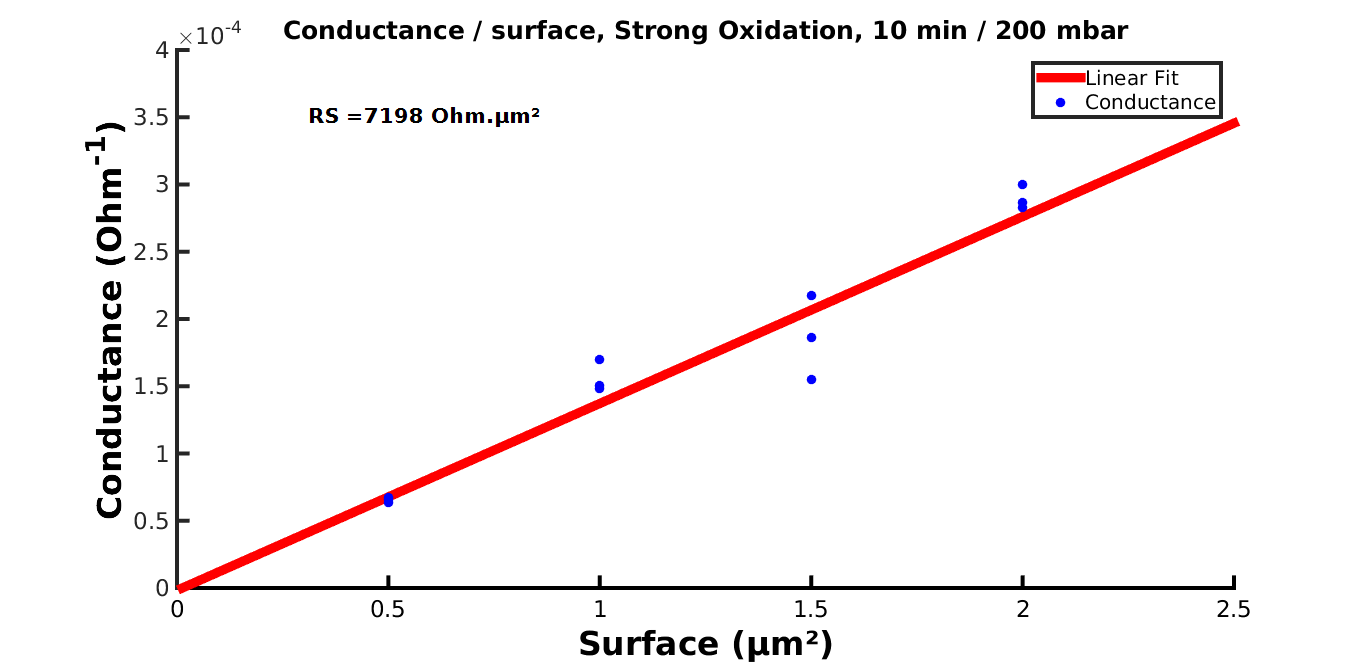
\includegraphics[width=15cm]{ConductanceFitStrongOx.png}
                    \caption{Conductance in function of surface area for a strong oxidized sample}
                    \label{Strongox}
                \end{figure}
                
                In order to cover a large range of resistance, the third reference sample is also a tunnel junction but lighter than the previous one (2min at an oxygen atmosphere of 2mbar).
                
                Again, it is more relevant to draw the conductance (See Fig. \ref{Regularox}) to determine the RS parameter.
                
                \begin{figure}
                    \centering
                    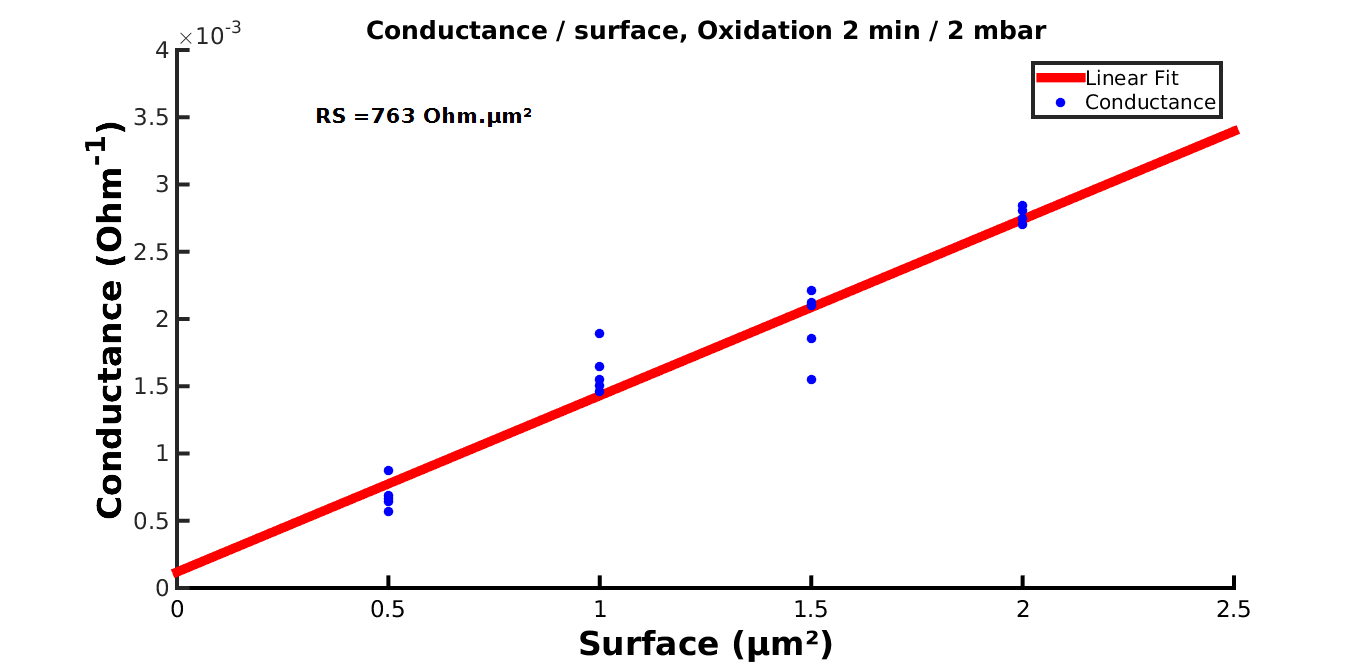
\includegraphics[width=15cm]{ConductanceFitOx.png}
                    \caption{Conductance in function of surface area for a tunnel junction sample}
                    \label{Regularox}
                \end{figure}
                                
                \[RS=763\Omega.\mu m^2\]
                
                RS is ten times less important than for the strong oxidation. It means that the oxide layer is quite thinner in this case, which is normal since the Al was less oxidized in this case.
                These three references give us a base to evaluate the quantity of oxide we etch when we use the plasma.
                \subsection{Plasma Etching : Position of the sample}
                
                The first test to do with the plasma etching is to determine if the beam is focused on the whole sample stage (15cm diameter) and not only on the center. This information will ensure a good homogeneity of the etching on all the surface. In order to do so, four samples where placed on the sample holder : one in the center and three on the side (see inset of Fig. \ref{PlasmaPosition}). The layer of evaporated Al was strongly oxidized, then the oxidation layer was etched by argon plasma for 10 min. Finally, we have made a clean contact by evaporating Cu. The Figure \ref{PlasmaPosition} shows the results of these tests. We can see that the position does not affect the resistance of the sample so we can assume that the etching is quite uniform. And another conclusion of this graphe is that 10 min of plasma are enough to etch all the Al oxide : there is no surface dependance like for the oxidized samples and the resistance is about the same order of magnitude than the clean contact junction. The value is a bit higher because the plasma etches the oxide, so the Al layer is thinner (since AlOx is not deposed on top of Al), which reduce the surface section of the lead, thus, it increases the resistance.
              
                \begin{figure}
                    \centering
                    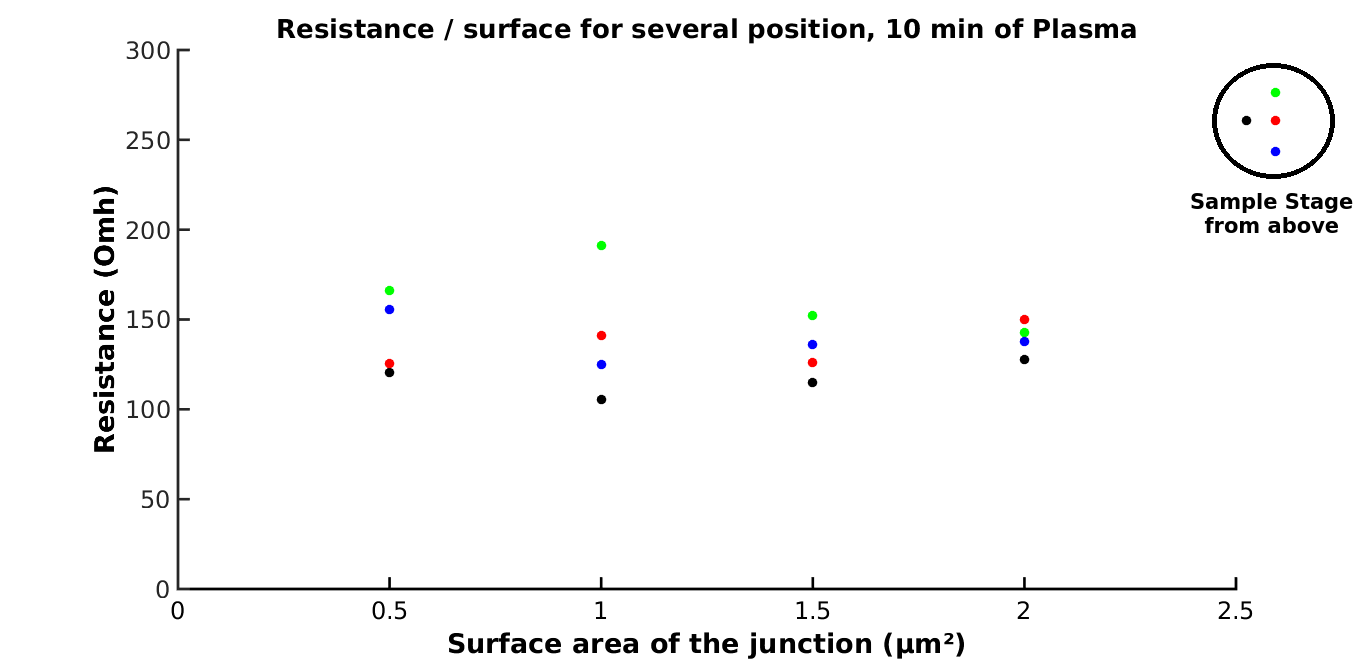
\includegraphics[width=15cm]{R_Position.png}
                    \caption{Resistance in function of surface for different positions of the samples on the LISA's sample stage}
                    \label{PlasmaPosition}
                \end{figure}               
                
                
                \subsection{Time of plasma etching}
                
                The time during which the sample is exposed to the plasma is important and determine how much materials will be etched and implicitely the resistance of the sample. The process is the same for all the samples, only the etching duration is modified.
                The Figure \ref{PlasmaTimeBefore} shows the resistance compared to plasma etching duration before the cleaning of the plasma gun. We can see that there is not a lot of differences between 10 and 20 minutes but the most relevant result is what we can see on the Figure \ref{PlasmaTimeAfter}, with samples made after the cleaning, it seems that less than 5 minutes are enough to etch all the oxide, since the results are very similar, yet for totally different duration times. It means that the cleaning had an effect on the plasma behavior.
                \begin{figure}
                    \centering
                    \begin{subfigure}[t]{0.99\textwidth}
                    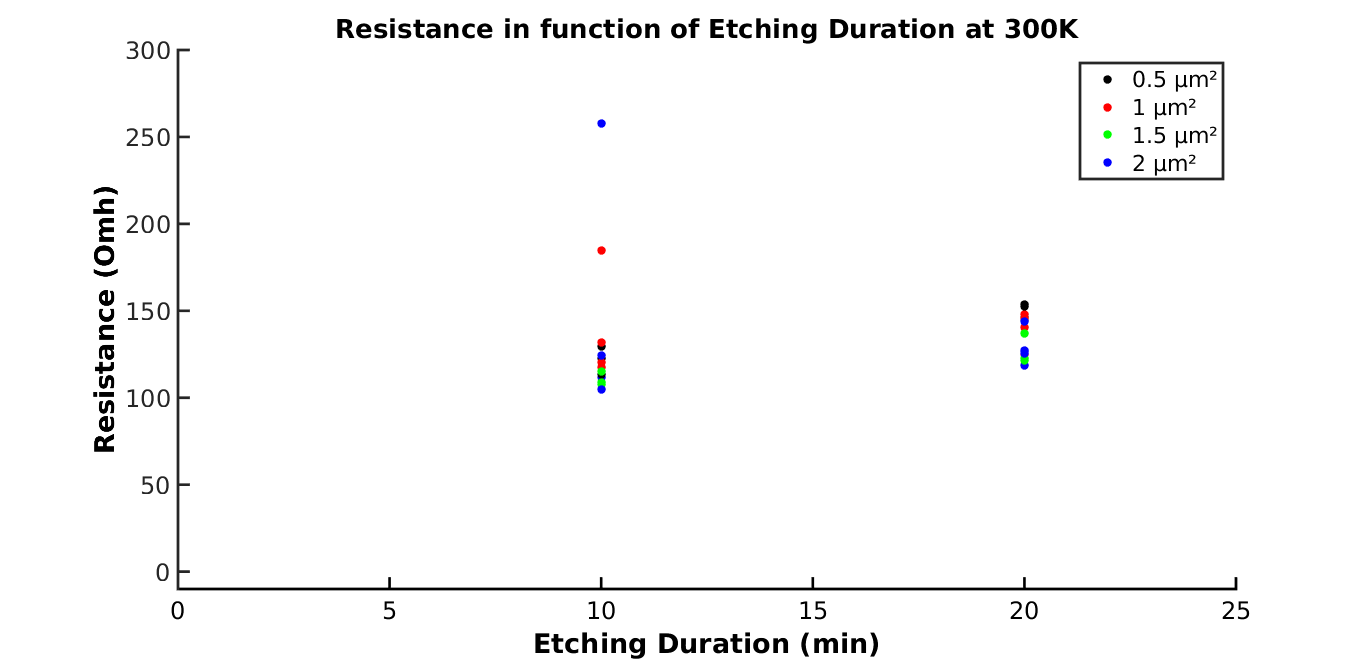
\includegraphics[width=14.9cm]{R_TimeBefore.png}
                    \caption{Resistance in function of Plasma Etching duration before the cleaning}
                    \label{PlasmaTimeBefore}
                    \end{subfigure}
                    ~
                    \begin{subfigure}[t]{0.99\textwidth}
                    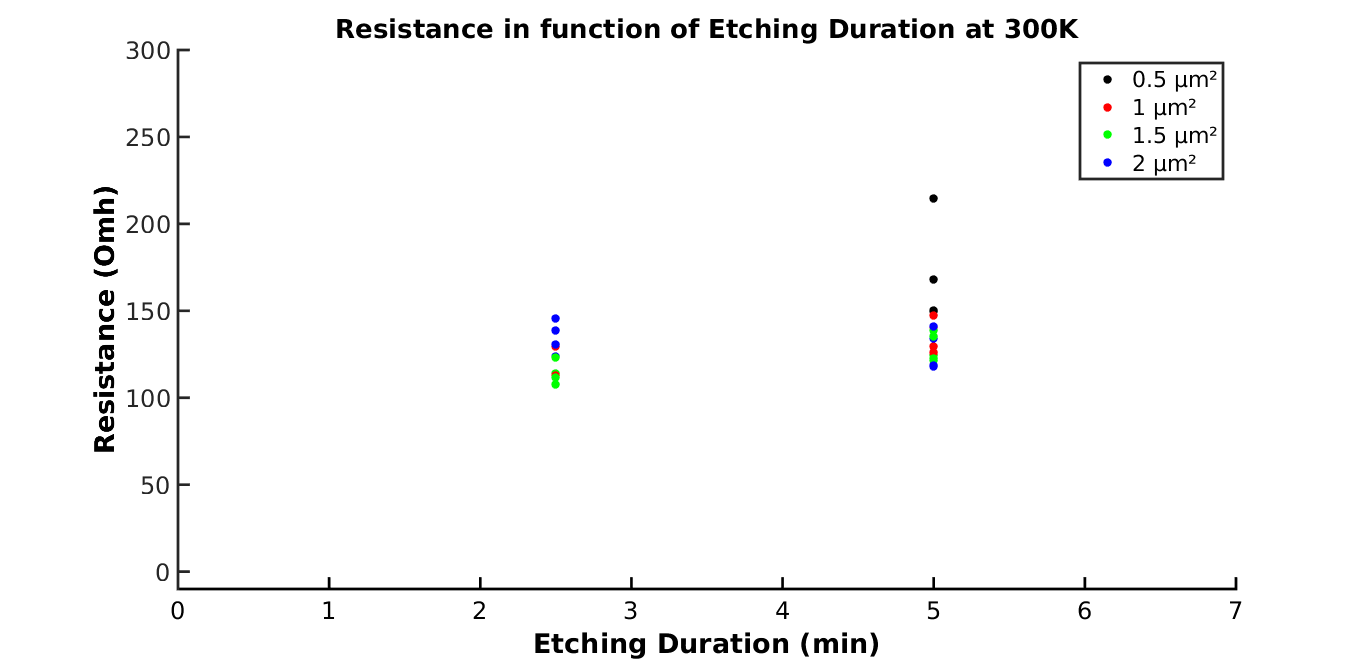
\includegraphics[width=14.9cm]{R_TimeAfter.png}
                    \caption{Resistance in function of Plasma Etching duration after the cleaning}
                    \label{PlasmaTimeAfter}
                    \end{subfigure}
                \end{figure}
                
            \subsection{Wafer Etching}
                According to the previous results, we can think that the oxygen cleaning made the plasma gun more powerful. Here is an observation that confirms this. The Figure \ref{WaferEtch} shows a SEM image of a sample exposed 10 minutes under the plasma after the oxygen cleaning. We can see that the plasma created a hole in the wafer, before the deposition of the copper above it.
                
            \begin{figure}
                \centering
                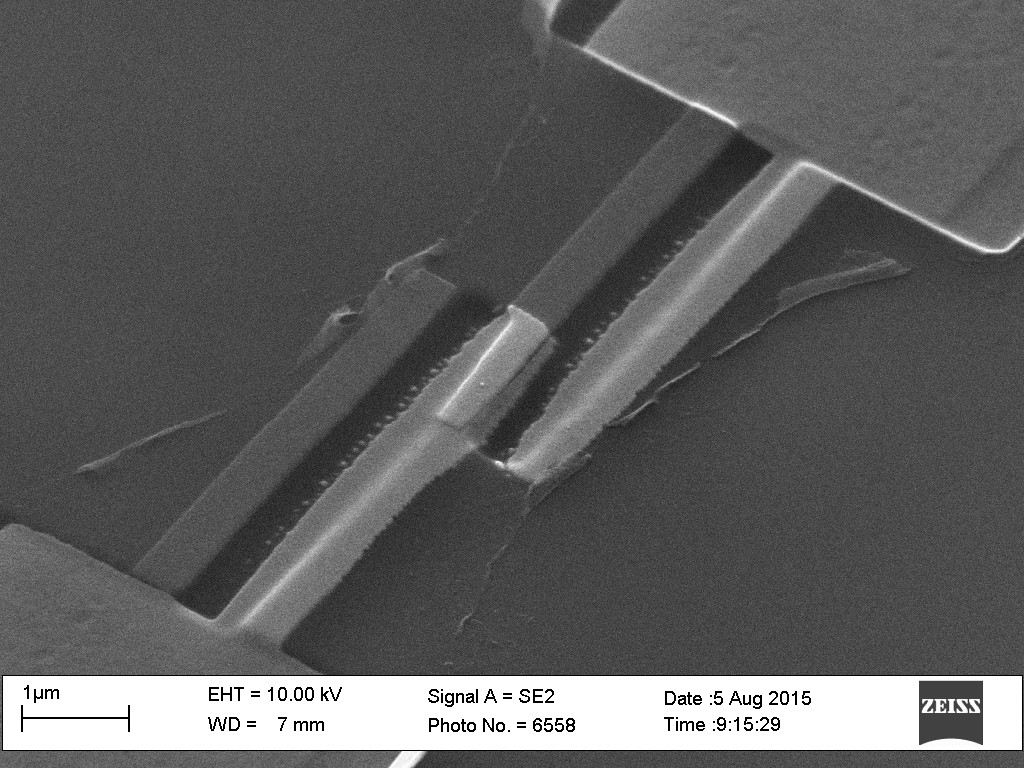
\includegraphics[width=250pt]{tiltSEM.jpg}
                \caption{SEM Image of a sample where the wafer was etched by plasma}
                \label{WaferEtch}
            \end{figure}
                
                \section{Low temperature measurements}
                
                \subsection{NIS Junction}
                
                The Figure \ref{IVlargeNIS} shows the I-V curve that was obtained at low temperature. The curve correspond to what the theory predicts. At a large range of $V_{bias}$ we see almost a strait line : there is tunneling when $V_{bias}$ goes over or under the threshold that the energy gap represents and a flat part in the middle when $V_{bias}$ does not reach the threshold. At a lower range of $V_{bias}$, closer to the limits of the tunneling, we can see (Fig. \ref{IVleakNIS}) better that the flat part is not constant : there is a leakage current, yet the slope is orders of magnitude below the tunneling current. But, there is another phenomenon visible : inside the leakage current there is a part that is steeper, which is the Andreev current, another transport phenomenon \cite{Andreev}.
                
                 The relation between the tunneling current and the leakage current is about 10$^{-4}$ which is quite good. These results are reproducible between different runs and samples. 
                
                \begin{figure}
                    \centering
                    \begin{subfigure}{\textwidth}
                    \centering
                    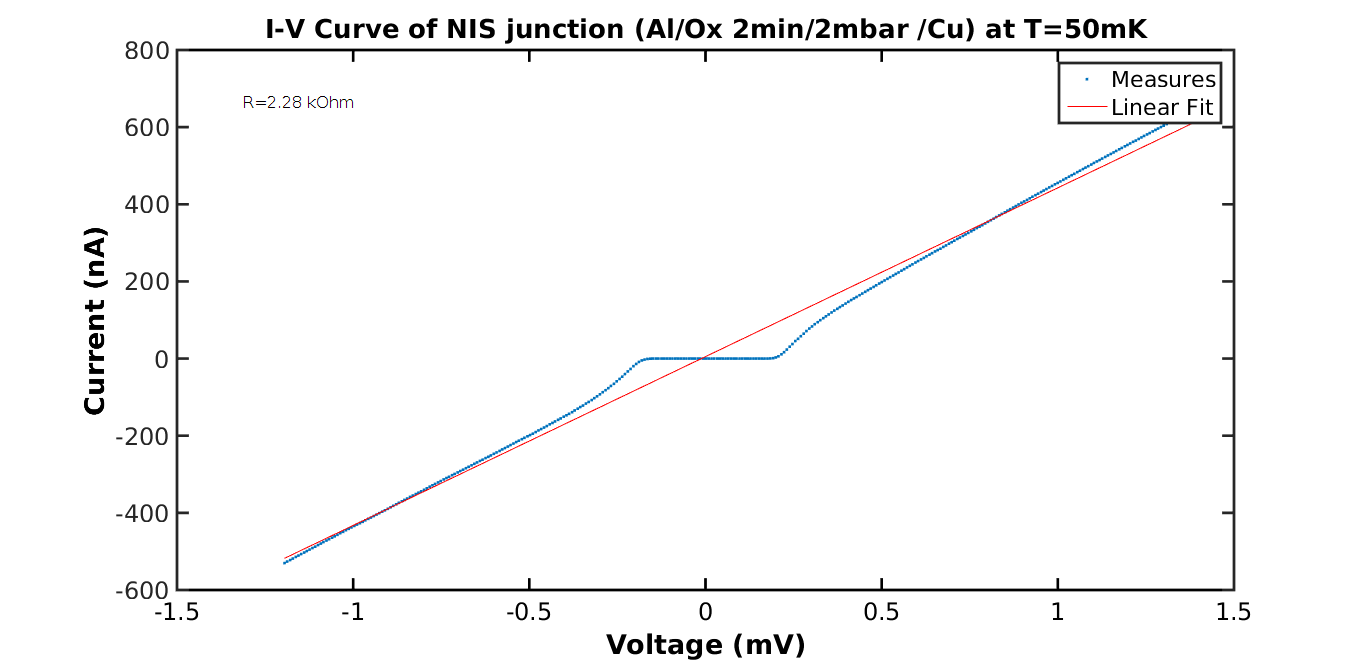
\includegraphics[width=15cm]{IVlargeNIS.png}
                    \caption{IV curve of NIS junctions with an oxidation under a pressure of 2mbar of O$_2$ during 2 minutes at 50mK}
                    
                    \label{IVlargeNIS}
                    \end{subfigure}
                    ~
                    \begin{subfigure}{\textwidth}
                    \centering
                    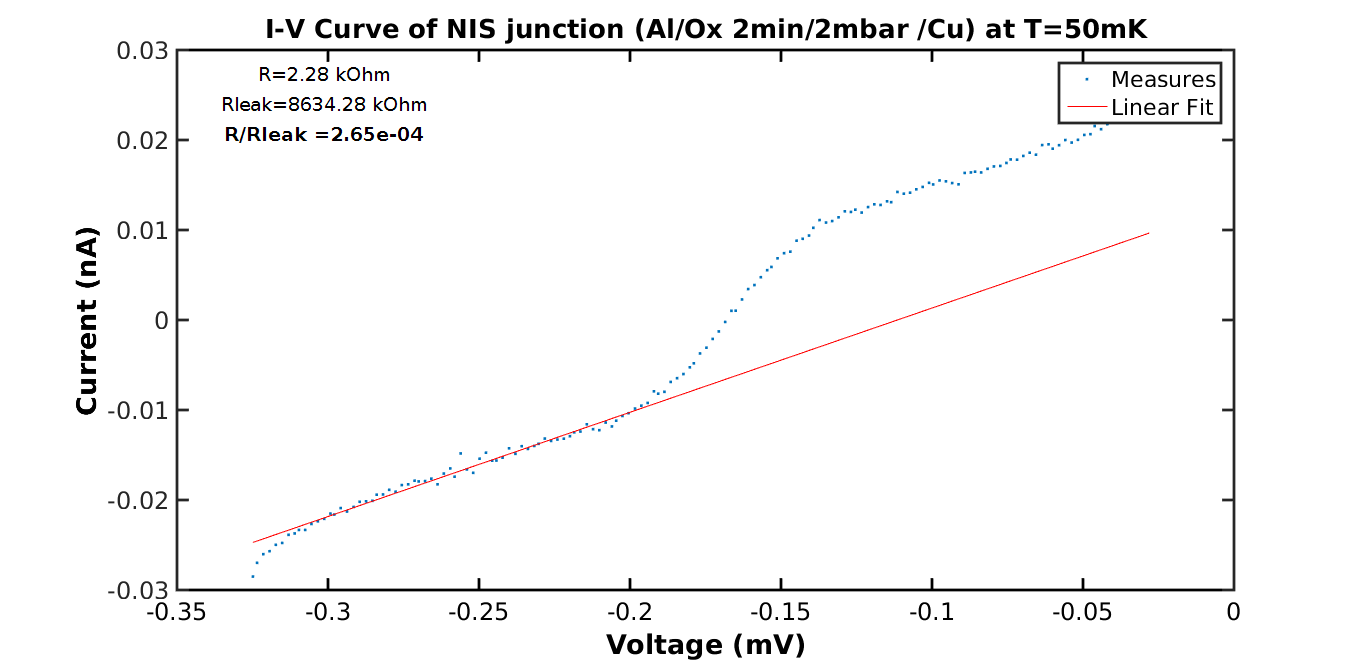
\includegraphics[width=15cm]{IVleakNIS.png}
                    \caption{Zoom in IV curve of NIS junctions with an oxidation under a pressure of 2mbar of O$_2$ during 2 minutes at 50mK}
                    \label{IVleakNIS}
                    \end{subfigure}
                \end{figure}
        
                Moreover, according to the theory, since the tunneling current is based on the density of states of the two material, if the temperature is modified, the current should be modified. Thermal agitation will have some effects on the I-V curves of the NIS junctions. Indeed, as we can see in Fig. \ref{Tsweep}, the coldest the junction is, the sharper the edges are. Heating will bring electrons in states above the Fermi level, and they will be able to tunnel, even if $|eV|<\Delta$.
                
                \begin{figure}
                    \centering
                    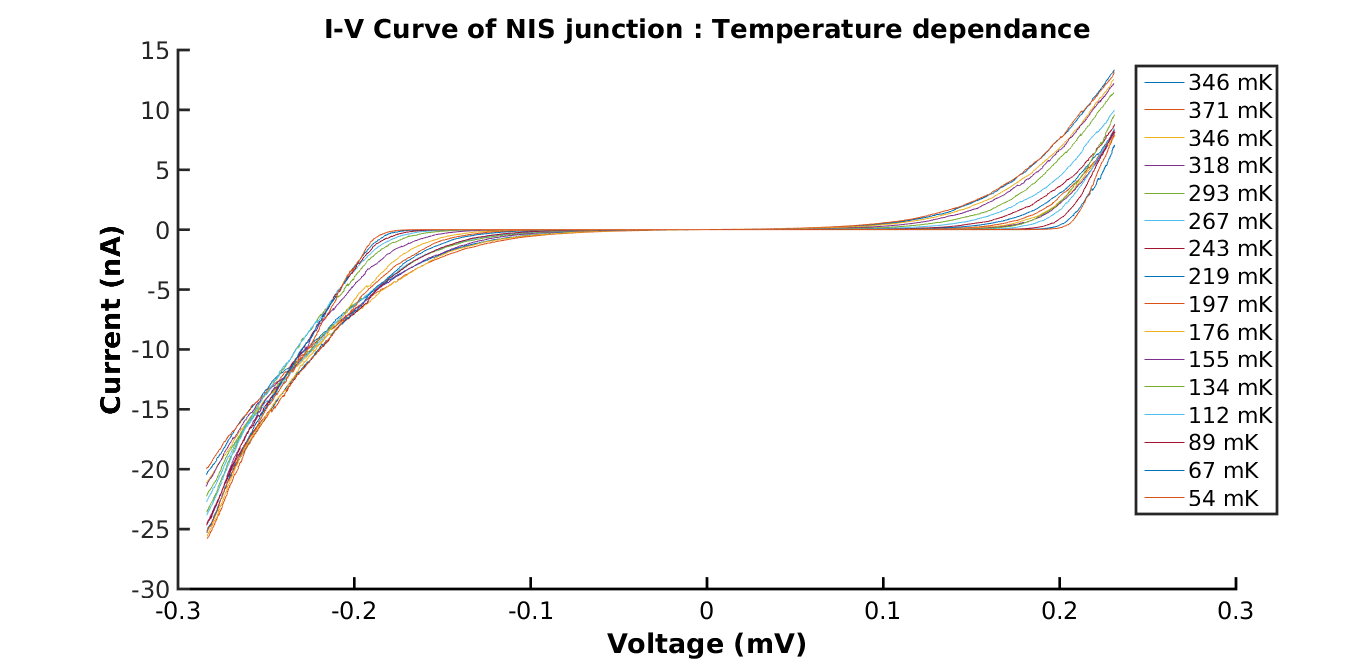
\includegraphics[width=15cm]{Tsweep.png}
                    \caption{Evolution of the IV curves of a NIS junction with the temperature}
                    \label{Tsweep}
                \end{figure}
                
                      
                \subsection{Plasma etched samples}
                This part shows the results of the samples where Al was strongly oxidize, then plasma etched and oxidized again to make a tunnel barrier. In order to discriminate the quality of the junctions by themselves, a reference sample was always done at the same time (without plasma etching and with tunnel barrier). Indeed, the junctions can be bad due to external reasons (polluted chamber, bad materials).
                The Figure \ref{PlasmaOx} shows the IV curves which were obtained for a plasma etched sample and the Figure \ref{ReferenceOx} show the correspondant regular oxidation reference for this sample.
         
        \begin{figure}
            \centering
            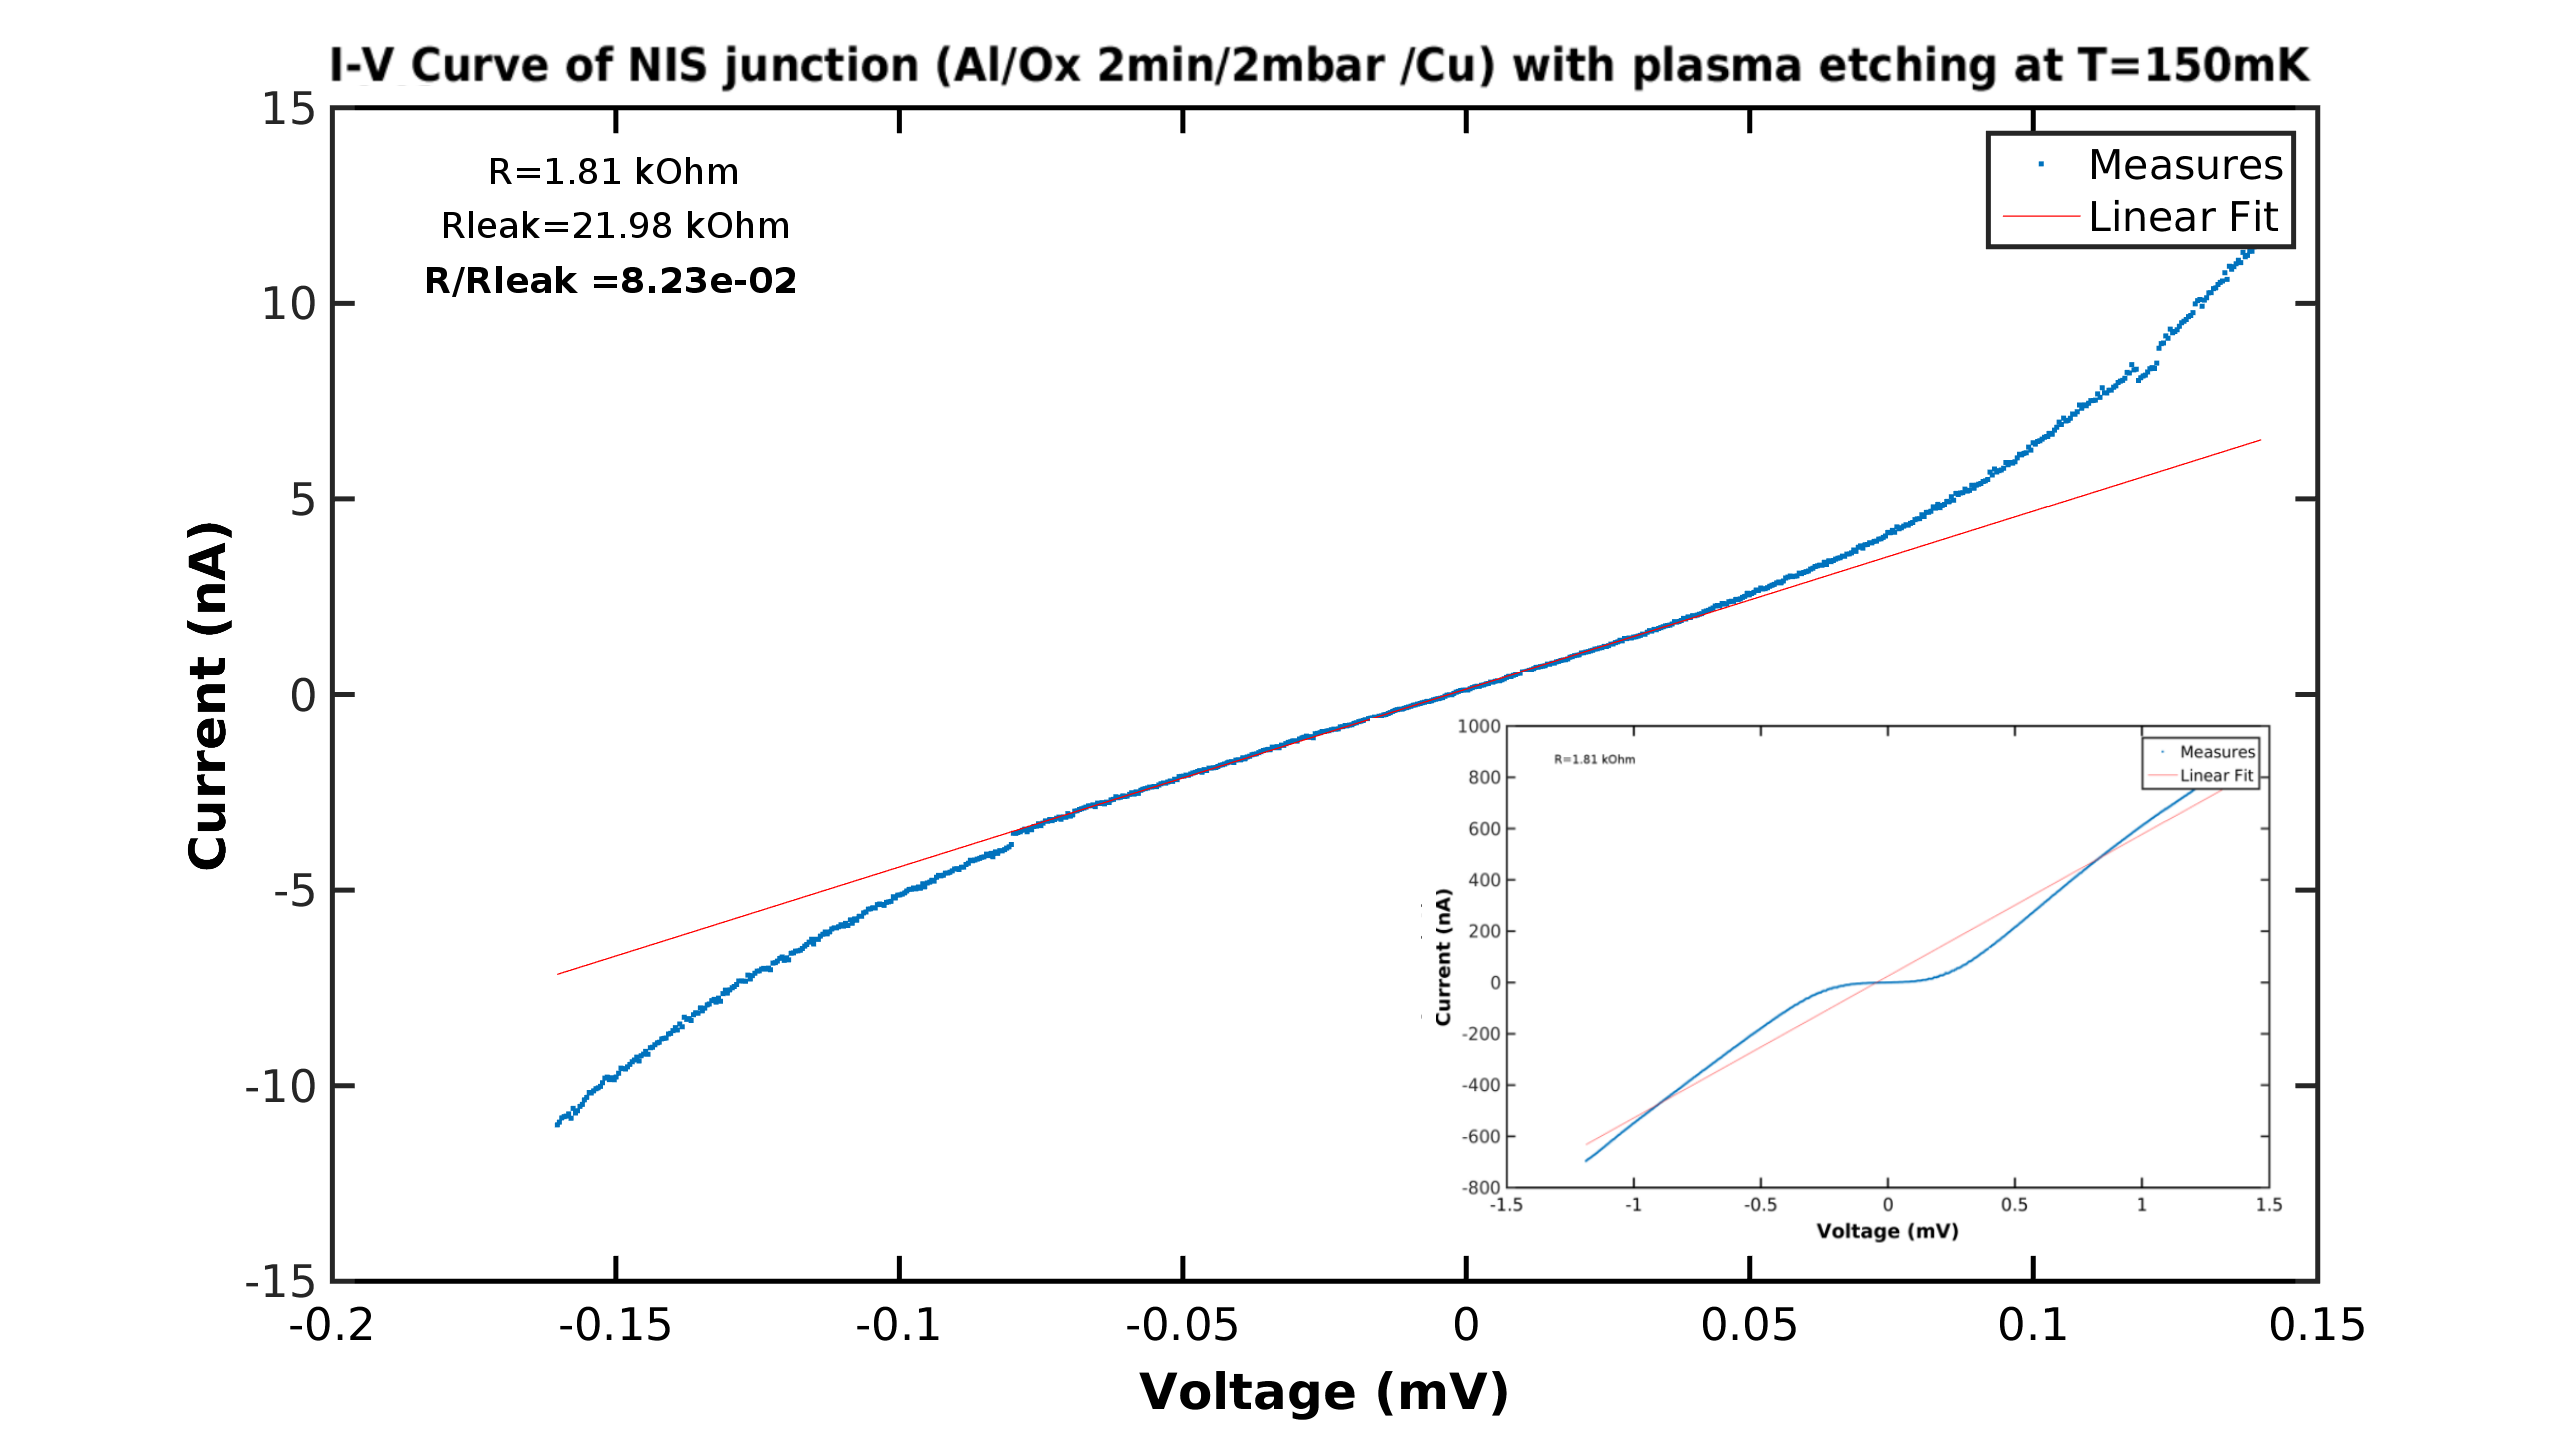
\includegraphics[width=15cm]{PlasmaOx2.png}
            \caption{IV curves of Plasma Etched sample}
            \label{PlasmaOx}
        \end{figure}
           \begin{figure}
            \centering
            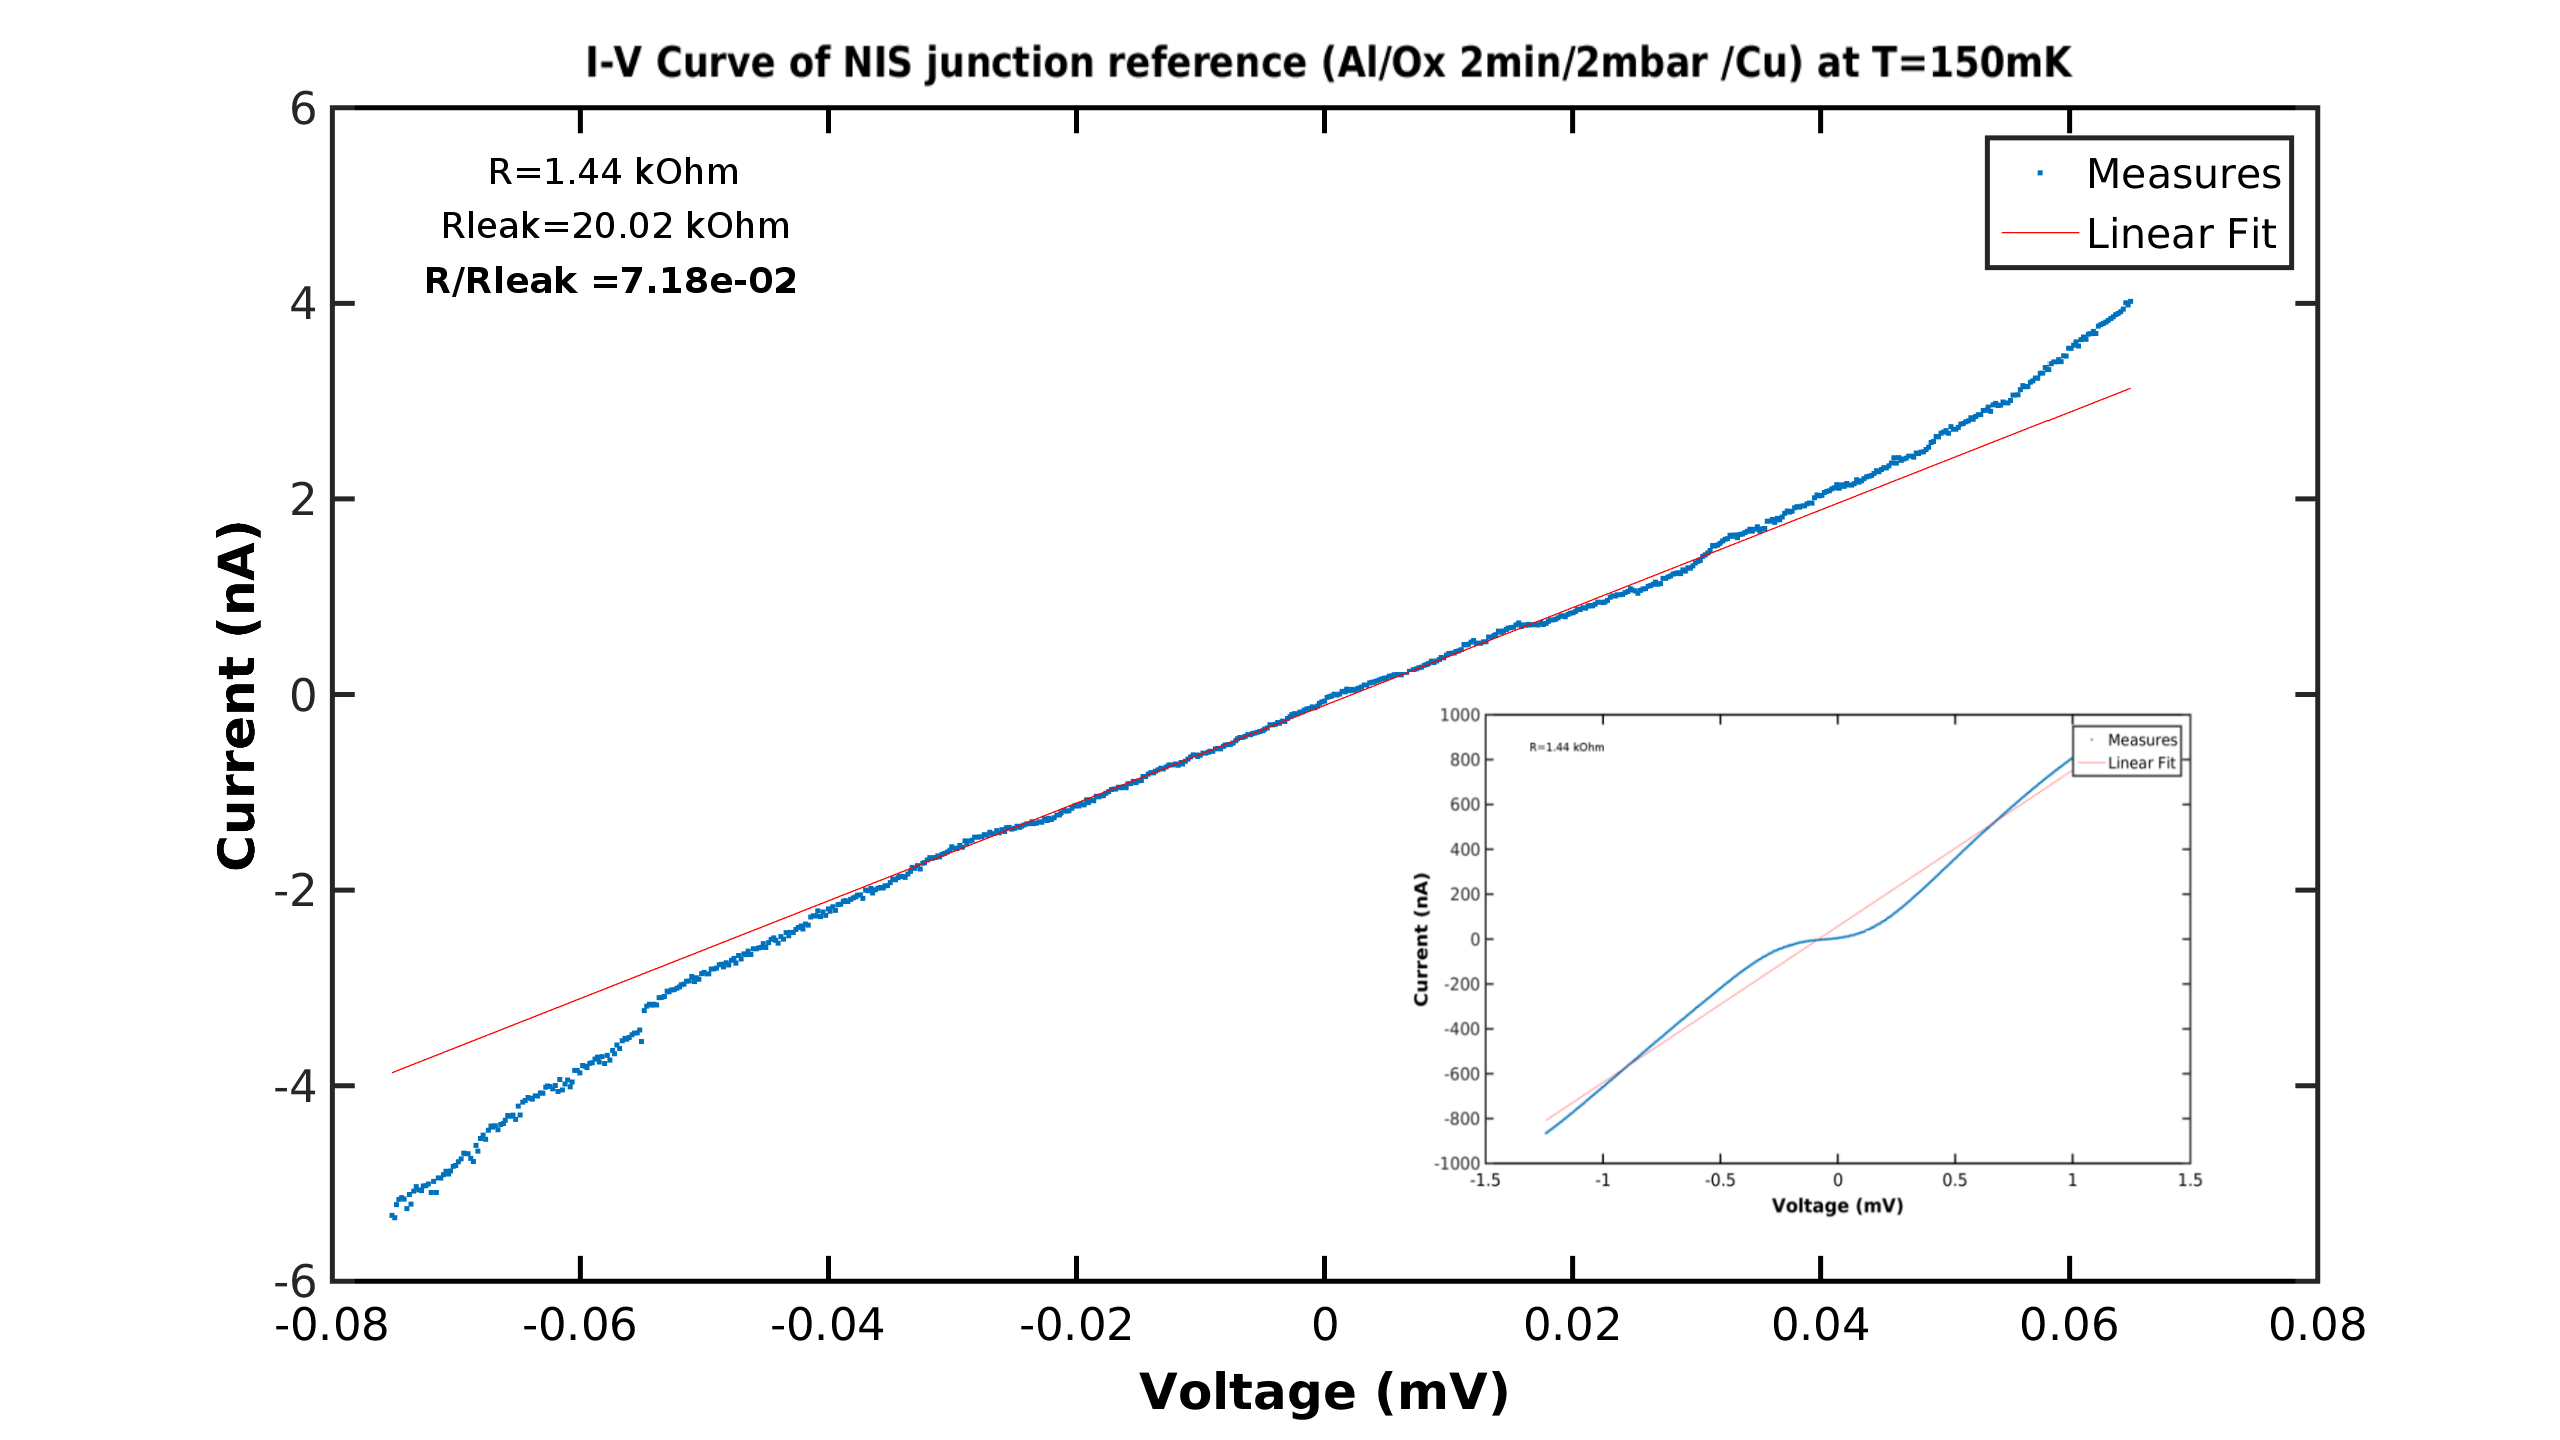
\includegraphics[width=15cm]{RegularOxRef2.png}
            \caption{IV curves of the reference oxidation sample}
            \label{ReferenceOx}
        \end{figure}
           
           We can see that the relation between the current is about the same order of magnitude in both cases : 10$^{-2}$. This is quite a bad result, but since the two relations are about the same value, we could think that the plasma does not damage the junction, but the effect of the plasma etching may be hidden behind the overall poor leakage of all the samples.
                
                \section{Summary of the results}
            
            Plasma etching is working fine, and can etch all the aluminium oxide without any visible damages on the junctions, plus the position of the sample on the sample stage does not affect the behaviour of the plasma etching. The question that has to be solved now is the effect of the plasma on the general quality of the junctions made in the evaporator : after heavy uses of the plasma, the quality of the junctions, in general, have degrading. Is it a coincidence or is it a collateral effect of the plasma ? This has to be solved but still not clear.
                
                
